\chapter{Implementation}

Mapping from one programming paradigm to another presents numerous challenges to the compiler writer. This section will highlight the main challenges encountered in the mapping from the object-oriented Dalvik executable format to the lower-level LLVM intermediate representation.

\section{Inheritance}

Object-oriented programming languages revolve around the ability for one class to reuse the behavior and attributes of another by \textit{inheriting} the data from a base class, also known as a superclass. The translation of this concept to LLVM bytecode proves a challenge to the compiler writer, since LLVM has no notion of classes. The closest that LLVM comes to having class behaviour  in the object-oriented sense comes through the use of structs.

Structs are analogous to the structs present in the C programming language; they are structured types that combine a set of fields into a single object. Much like the C structs (and unlike those found in C++), they are not permitted to have functions as struct members, nor do they directly support inheritance. These two omitted features are the biggest difference between structs and objects as found in objected-oriented languages.

Structs are, however, the closest LLVM comes to having `classes'. We must, therefore, manipulate these structs into representing the classes found in our Dalvik program. Fortunately there are ways around the shortcomings brought about by LLVM bytecode's low-level approach to code representation. Instead of associating methods with a class definition, methods are instead implemented globally in LLVM, without an associated object attached to them. To achieve the same functionality an object-specific method has with regards to the access of the object's attributes and other functions, LLVM methods are passed a `this' pointer if they are non-static. The pointer represents the instance of the class that the method intended to be a member of, allowing the method to access the correct data from that instance without breaking the priniciples of the object orientation paradigm.

The other challenge to tackle is that of object inheritance. Inheritance is effectively achieved through the same paradigm a C programmer might use to accomplish the same goal:

\lstset{
	language=C,
	basicstyle=\small,
	stringstyle=\ttfamily
}

\begin{lstlisting}[frame=single, numbers=left, numberstyle=\tiny, title=C code]
typedef struct {
    // base members
} Base;

typedef struct {
    Base base;  
    // derived members   
} Derived;

...

Derived *d;
Base *b = (Base *)d;
\end{lstlisting}

\begin{lstlisting}[frame=single, numbers=left, numberstyle=\tiny, title= LLVM IR]
%Base = type { /* base members */ }
%Derived = type { %Base, /* derived members */ }

...

%0 = alloca %Derived
%1 = bitcast %Derived* %0 to %Base*
\end{lstlisting}

We can see at line 6 of the C code - and at line 2 of the LLVM bytecode - that each struct features as its first field an instance of the super class. This way it can be cast to this class at runtime, as we do at lines 13 and 7 of each respective code sample. The object can then be used as if it were an instance of the super class, giving it access to the necessary data.




\section{Type Inference}

One feature of the Dalvik instruction set that poses a problem to the translation process is the Dalvik registers' ability to infer a value's type at run-time. Contrary to traditional, statically-typed languages, a value's type must be explicitly declared at compile time.

\lstset{
	language=C,
	basicstyle=\small,
	stringstyle=\ttfamily
}

\begin{lstlisting}[frame=single, caption={C example}, label=code:static]
int negate(int x) {
    int result; /* declare integer result */
    result = -x;
    return result;
}
\end{lstlisting}

As we can see from the example in the statically-typed C programming language in Listing \ref{code:static}, the return value of the \verb|negate| function must be declared alongside its type. The the bytecode for the Dalvik virtual machine, however, has no such constraint. For example, the instruction:

\lstset{
	language=Assembly,
	basicstyle=\small,
	stringstyle=\ttfamily
}

\begin{lstlisting}[]
const v0 0x3FF8000000000000
\end{lstlisting}

loads the constant literal hexadecimal value of \hex{0x3FF8000000000000} into register 0. At this point in the translation process, it is unknown what type of value this register contains - it is dependent on the manner in which it is treated: the value could either be the integer $4.6094342186137 \times 10^{18}$, or the floating-point value of 1.5, depending on the context in which the register value is used in instructions further on in the program.

LLVM intermediate representation does not feature such a notion. Each type must be explicitly declared statically at compile time, as in the C example shown in Listing \ref{code:static}. Upon occuring a Dalvik bytecode instruction similar to the one given above, we must be able to deduce its type in order to validly allocate it on the stack, store it there, and be able to load and use that value later in the program. This is information that the Dalvik instruction does not give us at the time it is needed. To this end, we must find a solution to the difference between how each language treats the types of its variables.

A simple solution to this problem would be to store the literal value of the constant upon finding such an instruction. Later in the program, when the constant value is used in a type-specific way, we could proceed to allocate the value onto the stack and store the literal value that we have been keeping aside. While this method solves the problem at hand, it is not the `cleanest' solution available. Most notably, it tampers with the original instruction order of the program, as the storing of the variable in the register would not occur at the point in the program at which Dalvik intended it.

We therefore propose an improved solution to the problem at hand. We introduce a dummy variable to a method's allocation stack, which serves as a `marker', to which we store temporary variables. To illustrate this with an example, consider an expanded example of the Dalvik instruction discussed earlier:

\begin{lstlisting}[frame=single, numbers=left, numberstyle=\tiny]
const v0 0x3FF8000000000000
add-float v1, v0, 3.5
\end{lstlisting}

As previously mentioned, at line 1, upon reading the first instruction, we can not infer the type of the value to be loaded into register 0. Seeing as we are unable to allocate the appropriate stack variable, we take note of the hexadecimal value of the constant, and store it in a hashmap in our internal representation. Additionally, we store 0 to our dummy variable, named \verb|%tmp|. This can be seen in Listing \ref{code:tmp1}.

\begin{lstlisting}[frame=single, numbers=left, numberstyle=\tiny, caption={LLVM bytecode}, label=code:tmp1]
define void @function() {
allocas:
  %tmp = alloca i8
label_0:
  store i8 0, %i8* %tmp ; Mark where the constant is found
}
\end{lstlisting}

We then arrive at the next instruction, the \verb|add-float| instruction, which adds two floating-point numbers and stores the result in a register. At this stage, we are able to infer that register 0 contains a floating-point value. Since register 0 is currently associated with a store instruction - the one of 0 to \verb|%tmp| - we know that it must contain a constant value. We can determine this because in normal circumstances a store instruction never returns a value.

Given that we now have information about the constant's type, we retrieve the hexadecimal value from the hashmap and allocate a new stack variable with the appropriate type. We then wish to store the constant to this newly-allocated variable. However, this leads us again to the problem highlighted above. The LLVM C++ API provides functionality that aids us in retaining the correct order of instructions when facing a Dalvik instruction that uses type inference. LLVM's API gives us the option of \textit{retrospectively replacing} an earlier instruction with another one. Since the variable associated with register 0 in our intermediate representation is currently pointing to a store instruction, we can replace it with another store instruction, based on our new knowledge of the variable's type. This new instruction stores the literal value - decoded from the hexadecimal according to the type information - to the newly-allocated stack variable.

\begin{lstlisting}[frame=single, numbers=left, numberstyle=\tiny, caption={LLVM bytecode}, label=code:tmp2]
define void @function() {
allocas:
  %tmp = alloca i8
  %v0 = alloca float
label_0:
  store float 1.5, %float* %v0 ; Replace tmp store
  ... ; carry out the float-add instruction
}
\end{lstlisting}

As shown here in the LLVM Bytecode Listing \ref{code:tmp2}, the original `dummy' store to the variable \verb|%tmp| on line 5 of Listing \ref{code:tmp1} has been retrospectively replaced with the store to the float pointer on line 6.

The original \verb|%tmp| allocation can then later be optimized out of the LLVM module, as it will not be used by any instruction at the end of the translation.


\section{Dynamically-typed Registers}
\label{sec:dyntype}

In a similar vain to the problem of Dalvik value type inference detailed in Section \ref{sec:typeinf}, there exists another difference between how Dalvik and LLVM handle register types. Dalvik registers are all 32-bit wide, and are not required to contain one particular type for the duration of the program. A register that contains an integer can hold a floating-point value sometime later in the program. 

To illustrate this example, let us consider how Dalvik might translate the following Java code snippet:

\lstset{
	language=Java,
	basicstyle=\small,
	stringstyle=\ttfamily
}

\begin{lstlisting}[frame=single, numbers=left, numberstyle=\tiny, caption={Java Dynamic Typing}, label=lst:java_dyn]
int x = 0;
int y = x + 1;
float z = 5.0f;
\end{lstlisting}

The Dalvik compiler might translate this example into the following Dalvik bytecode instructions:


\lstset{
	language=Assembly,
	basicstyle=\small,
	stringstyle=\ttfamily
}

\begin{lstlisting}[frame=single, numbers=left, numberstyle=\tiny, caption={Dalvik bytecode for Listing \ref{lst:java_dyn}}, label=lst:dalvik_dyn]
const v0, 0
add-int/lit8 v1, v0, 1
const v0, 4014000000000000
\end{lstlisting}

Here, in Listing \ref{lst:dalvik_dyn}, we load the constant value 0 into \verb|v0| on line 1, which corresponds to setting \verb|x = 0| on line 1 of Listing \ref{lst:java_dyn}. We proceed to add the literal value 1 to \verb|v0| and store that result into register \verb|v1|. This corresponds to the instruction on line 2 of Listing \ref{lst:java_dyn}. At this point in the program, register \verb|v0| is no longer needed, and can be used to hold another value. Hence, at line 3 of the Dalvik code we load the constant floating-point value 5.0 into the free register \verb|v0|. We have just moved a floating-point number into a register that previously contained an integer value.

This dynamic typing of registers is another feature of the Dalvik virtual machine that does not translate directly into LLVM bytecode. Once we declare and allocate a value of a certain type onto the stack, we are unable to store a value of a different type to that variable, without prior casting. It is illegal even to save a 16-bit integer to a 32-bit integer on the stack without bitcasting it first.

Let us now imagine we are traversing our internal representation whilst translating the Dalvik bytecode in Listing \ref{lst:dalvik_dyn} to LLVM intermediate representation.

\begin{lstlisting}[frame=single, numbers=left, numberstyle=\tiny, caption={LLVM IR for Listing \ref{lst:dalvik_dyn}}, label=lst:llvm_dyn] 
define void @function() {
allocas:
  %v0 = alloca i32
  %v1 = alloca i32
label_0:
  store i32 0, i32* %v0
  %t1 = load i32 %v0
  %t2 = add i32 %t1, i32 1
  store i32 %t2, i32* v1
}
\end{lstlisting}

We have hereunto translated up to line 2 the Dalvik bytecode in Listing \ref{lst:dalvik_dyn}. We now come across line 3, the floating-point store instruction. Let us assume that we know that this store instruction is of floating-point type (see Section \ref{sec:typeinf} for an explanation as to why this is not necessarily the case at this stage in the program). We wish to store the value 5.0 to the value pointed to by register \verb|%v0| in our internal representation, as the Dalvik bytecode commands. However, this register variable points to an allocation of type \verb|i32|, a 32-bit integer. Storing a floating point value to this type would result in an invalid LLVM module.

We therefore must check the type pointed to by the allocation instruction, and check it against the type that we wish to store. If the types are not equal then we must allocate a new variable on the stack with the appropriate type, then point the register variable in the internal representation to this new allocation for future instructions to refer to.

\begin{lstlisting}[frame=single, numbers=left, numberstyle=\tiny, caption={LLVM IR for Listing \ref{lst:dalvik_dyn} (cont.)}, label=lst:llvm_dyn2]
define void @function() {
allocas:
  %v0 = alloca i32
  %v1 = alloca i32
  %v0_2 = alloca float
label_0:
  store i32 0, i32* %v0
  %t1 = load i32 %v0
  %t2 = add i32 %t1, i32 1
  store i32 %t2, i32* v1
  store float 5.0, float* %v0_2
}
\end{lstlisting}

As shown in the updated version of the LLVM bytecode, Listing \ref{lst:llvm_dyn2}, we have allocated a floating-point type on the stack, and stored the constant value to that. Register \verb|%v0|, as it is represented internally, now points to the new allocation, \verb|%v0_2|, and the old allocation \verb|%v0| is no longer accessible. This is an unfortunate consequence of the method used to deal with the translation of dynamic register types. For example, if the register was later to be used to store another integer, it would be ideal to be able to go back to using the old integer definition of \verb|%v0| instead of allocating another integer on the stack and using that. Fortunately, LLVM's comprehensive suite of optimisations reduces some of the penalty induced here, for example using constant propagation to eliminate a lot of the allocations, stores and loads of constant values that are common in user programs.


\section{Register Mapping}


\section{The Stack}
\label{sec:stack}

LLVM intermediate representation is written in static single assignment (SSA) form. This property states that each variable is assigned exactly once, with variables being split into versions, with every variable receiving its own definition. The motive behind SSA form is that it simplifies and improves the results of various compiler optimisations, by more explicitly stating data dependencies. The Dalvik executable format, however, is register-based, so we have no need for SSA form while generating code. Our values are held in a fixed set of registers, and when a value is written to, we can no longer access the old value, nor do we need to.

To this end, we instead allocate mutable variables on the stack and use load and store instructions to access them. In LLVM, all memory accesses are explicit with load/store instructions. Every read of a value then becomes a load from the stack, and each update of a variable becomes a store to the stack. This paradigm introduces a problem, however; we now introduce a lot of stack traffic for simple and commonplace operations. This is evidently a major performance issue. The LLVM optimiser has a solution to this problem: the `mem2reg' pass. This optimisation promotes memory accesses to register variables and tidies up the loose ends. This is a high-performance optimisation that is used by major LLVM frontends such as clang and llvm-gcc\footnotemark \footnotetext[1]{http://llvm.org/docs/tutorial/LangImpl7.html\#memory}. We therefore rely on this optimisation pass to keep the generated code performing well.

Care must be taken when traversing a Dalvik method whilst translating it into LLVM bytecode in this way, however. If we translate from Dalvik to LLVM bytecode na\"{\i}vely, allocating a register variable on the stack as soon as we come across it, we run into major problems, specifically when control-flow comes into play.

Let us now consider a simple example in which a problem might arise. Take the sample Java snippet:

\lstset{
	language=Java,
	basicstyle=\small,
	stringstyle=\ttfamily
}

\begin{lstlisting}[frame=single, numbers=left, numberstyle=\tiny, caption={Java control-flow example}, label=lst:java_br]
int x;
if (a < b)
    x = 0;
else
    x = 1;
return;
\end{lstlisting}

and its Dalvik translation:

\lstset{
	language=Assembly,
	basicstyle=\small,
	stringstyle=\ttfamily
}

\begin{lstlisting}[frame=single, numbers=left, numberstyle=\tiny, caption={Dalvik code for Listing \ref{lst:java_br}}, label=lst:dalvik_br]
if-ge a, b, 4
const x, 0
return void
const x, 1
goto 3
\end{lstlisting}

In Listing \ref{lst:dalvik_br}, the branch targets in the \verb|if-ge| and \verb|goto| instructions are absolute, and refer to the line numbers at the left of the code frame. Additionally, this section of Dalvik bytecode might be represented by the control-flow graph (CFG) in Figure \ref{fig:cfg_dalvik}.

Looking at the example in Listing \ref{lst:dalvik_br}, we see the order of instructions that our compiler's code generation component will process. We are also able to see the basic blocks in which each instruction resides from Figure \ref{fig:cfg_dalvik}. After translating the branch instruction, we come across the instruction on line 2 of Listing \ref{lst:dalvik_br}; the store of the constant 0 to the variable \verb|x|. We are currently generating instructions from within the basic block on the left.

\begin{figure}[h!]
    \centering
    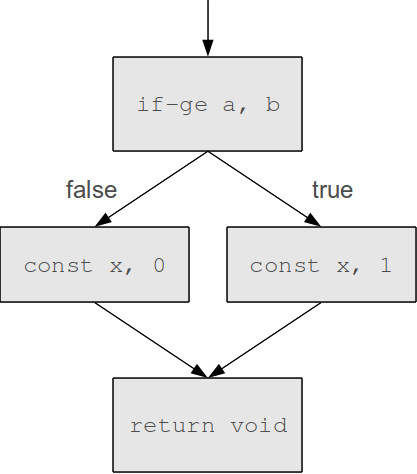
\includegraphics[width=0.4\textwidth]{images/cfg_dalvik.png}
    \caption{CFG representation of Listing \ref{lst:dalvik_br}}
    \label{fig:cfg_dalvik}
\end{figure}

Assuming that we have not seen the variable \verb|x| before, we create a new integer allocation on the stack in which we store the appropriate value. Generating code na\"{\i}vely, we have placed the allocation inside the basic block in which we reside. By the time that we come to the second store instruction we have moved into the basic block on the right of Figure \ref{fig:cfg_dalvik}. The variable \verb|x| has been previously discovered and handled by the code generator, and so we do not need to create another allocation. We continue, store the value 1 into the variable, and the complete the translation from Dalvik to LLVM bytecode. The CFG associated with this generated section of LLVM bytecode is detailed in Figure \ref{fig:cfg_llvm}.

\begin{figure}[h!]
    \centering
    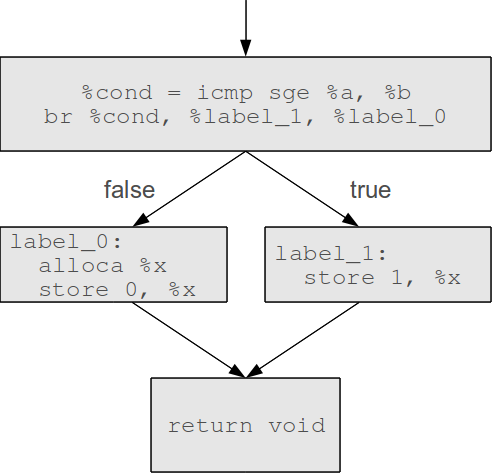
\includegraphics[width=0.5\textwidth]{images/cfg_llvm.png}
    \caption{CFG for the LLVM bytecode of Listing \ref{lst:dalvik_br}}
    \label{fig:cfg_llvm}
\end{figure}

However, there is a major problem with this resulting LLVM module. The allocation that we created in the first basic block does not dominate all of its uses. For example, if the condition on the branch instruction was true, i.e., \verb|a| was \textit{not} strictly less than \verb|b|, then the program would jump into the latter basic block - skipping the first entirely - and attempt to store a value to an as-of-yet unallocated variable \verb|x|. This is evidently a major error in the module, and the program would segmentation fault if run.

One solution to this pitfall is to create all allocations in a place where they dominate all subsequent instructions, i.e., they have function-wide scope. Therefore we introduce a new basic block to the start of every method, in which we carry out all stack allocations, in order to ensure that they have function-wide scope. We name this basic block \verb|allocas|, and it will feature in all subsequent LLVM bytecode listings. The unconditional branch from the allocation block to the first block of the method will be omitted, to avoid cluttering an example.

The corrected LLVM module of this example is shown in Figure \ref{fig:cfg_llvm2}, where the allocation of the variable \verb|x| is moved up to the dominator block at the beginning of the function. In this way we can guarantee that all load and store instructions to this variable are legal.


\begin{figure}[h!]
    \centering
    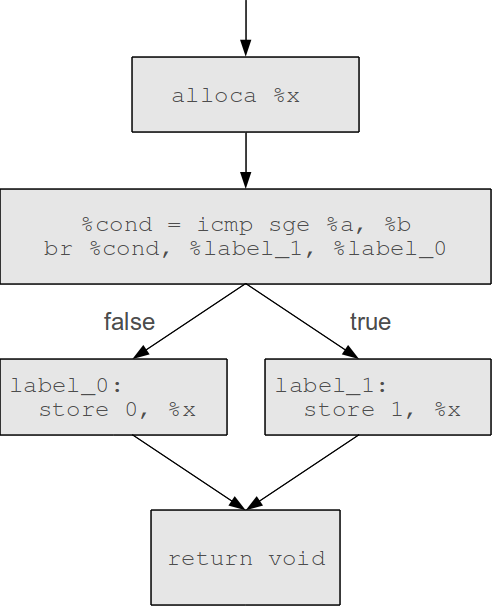
\includegraphics[width=0.5\textwidth]{images/cfg_llvm2.png}
    \caption{CFG for the corrected LLVM bytecode of Listing \ref{lst:dalvik_br}}
    \label{fig:cfg_llvm2}
\end{figure}



\section{Arrays}
\label{sec:arrays}

Given the widespread use of arrays in computer programs, it is no surprise that they are encountered frequently when translating Dalvik bytecode to LLVM intermediate representation. Once again there is disparity between how the two languages handle these data structures, stemming from the difference between the two programming paradigms that they adhere to. The generation of correct and efficient array code is key to achieving good performance in any compiler.

LLVM has two methods for handling array representations. The first is the aggregate array type, a form familiar to the high-level programmer:

\lstset{
	language=Assembly,
	basicstyle=\small,
	stringstyle=\ttfamily
}
\begin{lstlisting}[frame=single]
%array = [<# elements> x <element type>]
\end{lstlisting}

The second is to represent arrays using pointers, as C or C++ programmers might be accustomed to:

\begin{lstlisting}[frame=single]
%array = <element type>*
\end{lstlisting}

Similar to the C programming language, these two representations of arrays are equivalent, as an array decays into a pointer to its first element. There are, however, differences between these two representations, and each has their own suitabilities for certain applications. We need to weigh up these options before we decide how to implement Dalvik arrays in LLVM bytecode. Let us consider the arrays we deal with, and examine how they are used in a Dalvik executable program.

We can encounter arrays in Dalvik programs in one of two ways: the first is when they are declared and defined in a method body. Shown in Listing \ref{lst:java_array1} are two examples of creating new arrays inside a Java method. Notice how in both cases we are directly specifying a length for each array within the defintion, whether explicitly or implicitly as in the former and latter definitions, respectively.

\lstset{
	language=Java,
	basicstyle=\small,
	stringstyle=\ttfamily
}
\begin{lstlisting}[frame=single, caption={Java arrays}, label={lst:java_array1}]
int a[] = new int[3];   // Declare
int b[] = {1, 2, 3};    // Declare and initialize with literal
\end{lstlisting}

The second way in which arrays can feature in Dalvik executable programs is when they exist as members of a class definition. Listing \ref{lst:java_array2} gives an example of an array being declared and defined as a private member of the class \verb|MyClass|:

\begin{lstlisting}[frame=single, caption={Java arrays}, label={lst:java_array2}]
class MyClass {
  private int a[] = {1, 2, 3};
  MyClass() { } // Class constructor method
}
\end{lstlisting}

Although we are once again implicitly specifying the array's length in the definition of this class variable, there one important distinction: Dalvik only handles the \textit{declaration} at class-level, implementing the definition inside the constructor method. This means that the array length is unknown to us as we come across its definition in the class data section of the Dalvik executable file. In the constructor method for the class, a local fixed-length array (similar to the ones in Listing \ref{lst:java_array1}) is created then `pushed' to the appropatie class variable.

We are left with a choice as to how we represent and implement both types of array in LLVM bytecode. The natural and most intuitive way of representing arrays of the sort shown in Listing \ref{lst:java_array1} is to equate them with the fixed-length LLVM arrays, as their length is specified at declaration-time. This form not only holds the length information in the array, but handles the memory management for us too, allocating enough memory for all array elements.

\lstset{
	language=Assembly,
	basicstyle=\small,
	stringstyle=\ttfamily
}

\begin{lstlisting}[frame=single, caption={LLVM fixed-length array}, label=lst:llvm_fix]
%a = [3 x i32]
\end{lstlisting}

The second sort of arrays, those without a known length at declaration-time, could indeed be represented by the same notation as those with a fixed length. LLVM allows arrays to be declared with a length of 0 to indicate a variable-sized array.

\begin{lstlisting}[frame=single, caption={LLVM variable-length array}, label=lst:llvm_var]
%a = [0 x i32]
\end{lstlisting}

Unlike arrays that are declared with a size associated with them, the variable-length array declaration does \textit{not} allocate enough memory for its elements, so we need to implement the memory management for such arrays ourselves. Memory allocation comes in the form of the \verb|malloc| function, which works in the same way as the version from the C programming language. Once we have learned the length of array - but after the initial declaration - we need to allocate enough memory on the heap for the entire array.

The following examples detail code from the C programming language (Listing \ref{lst:malloc_c}) and its translation into LLVM bytecode (Listing \ref{lst:malloc_llvm}). We declare a pointer to an integer, which is analogous to a variable-length array, as explained earlier in the Section. Later in the program, once we learn of the length we want to give this array - 3 in our case - we call the \verb|malloc| function enough space for $3 \times sizeof(int)$, or 12 bytes. We must then cast the result to an integer pointer and store it in our array variable:

\lstset{
	language=C,
	basicstyle=\small,
	stringstyle=\ttfamily
}
\begin{lstlisting}[frame=single, numbers=left, numberstyle=\tiny, caption={C malloc}, label=lst:malloc_c]
int* a;
void* res = malloc(3 * sizeof(int));
int* cast_res = (int*)res;
a = cast_res;
\end{lstlisting}


\lstset{
	language=Assembly,
	basicstyle=\small,
	stringstyle=\ttfamily
}
\begin{lstlisting}[frame=single, numbers=left, numberstyle=\tiny, caption={LLVM malloc}, label=lst:malloc_llvm]
%a = alloca i32*
%res = call noalias i8* @malloc(i64 12) nounwind
%cast_res = bitcast i8* %res to i32*
store i32* %cast_res, i32** %a
\end{lstlisting}

The C code in Listing \ref{lst:malloc_c} uses a pointer to represent a variable-length array, and so we choose to do the same in our LLVM bytecode translation. The pointer representation is more intuitive and more closely-resembles the memory-allocation paradigm used by other programming languages over the variable-length array notation given earlier. We now have two representations for the two different types of array, the fixed-length array notation (Listing \ref{lst:llvm_fix}) for constant and fixed-length arrays, and pointer notation (Listing \ref{lst:llvm_ptr}) for variable-length arrays whose size are unknown at declaration-time.

\begin{lstlisting}[frame=single, caption={LLVM pointer array}, label=lst:llvm_ptr]
%a = i32*
\end{lstlisting}

When it comes to assigning data values to the now-allocated variable-length array, we `copy' a local fixed-length array to it. At this point the disparity between Dalvik and LLVM bytecode shows itself once again. In Dalvik bytecode we simply call the \verb|iput-object| instruction, which copies the register containing our local array to another register containing the target class variable.

LLVM does not provide such functionality for us, being a lower-level representation. In order to copy a block of memory to another we use the LLVM llvm.memcpy instrinsic function. One of the function's parameters is the number of bytes to copy over the the destination. We naturally want to copy the entire array over to our variable-length array, however, we no longer have the information on the length of the array to copy, as the current instruction, the \verb|iput-object| instruction provides no such data.

Note that in this example we \textit{do} have sufficient data to be able to infer the length of the array to copy, as the source is a fixed-length array. However, the \verb|iput-object| instruction is used in many other applications, including when we want to put a variable-length array to another. We want to be able to abstract this instruction and cover all cases in which it is used.


We therefore need a method by which we can always determine the size of an array at every reference to it. The solution is to combine a field containing the length of the array with the data structure itself. As soon as we learn of an array's length, we store it in the `size' field, and all subsequent instructions involving the array can access the length in order to perform bounds checking, to check how many bytes to allocate or copy, etc.

\lstset{
	language=Assembly,
	basicstyle=\small,
	stringstyle=\ttfamily
}
\begin{lstlisting}[frame=single]
%struct_array = { i32, i32* }
\end{lstlisting}

Given the more complicated memory management involved in implementing arrays in LLVM bytecode as opposed to Dalvik bytecode, several cutbacks were made. The first is that arrays of non-primitive types such as Objects are unsupported in this compiler prototype. Multidimensional arrays are also unsupported in order to provide more focus on other areas. These two array subtypes are entirely possible in LLVM, and would be important additions in future versions of the compiler.


%\section{Dalvik Executable Parsing}
\label{sec:parsing}

The first step in designing a compiler is naturally the parsing of the input language, which in our case is the Dalvik executable file format. On examining the file structure, we are able to see that the language is context-sensitive, according to the definition given by the Chomsky hierarchy of formal grammars. This is the case since each main section of data is located at a specific offset into the file, given in an initial header item. Furthermore, each section is broken down into subsections, all at offsets given elsewhere in the file. This means that we are unable to use the majority of parser generators for this section of the compilation process. These tools, which, given a formal definition of a language, generate the source code of a parser which can then be used as a component in the compiler toolchain. The drawback is that many of these are unable to handle context-sensitive languages.

% Code generator that can handle context-sensitive grammars?

It is therefore simpler that we design a custom parser for the Dalvik format which takes a Dalvik executable file as input and constructs an internal representation that we can pass on to the later components of the compiler. Hence, a custom parser is written in C++. The reason for using C++ is that we will be interfacing with the LLVM C++ API for generating code further down the line. The job of the parser is twofold: it traverses the input file in order, both keeping track of the various data sections it comes across for later use, and validating that the file is a valid Dalvik executable file.

As is evident from the structure presented in Table \ref{tab:dalvik_layout}, the file format is impossible to define in a context-free sense, given the self-referential nature of the format. This layout, however, renders it relatively straightforward to parse. It is a matter of traversing the input in accordance with the file structure as documented online \cite{dvk_format}, and keeping a track of the various data structures encountered along the way.

While most compilers must check that the source program adheres to the syntax of the language, we are able to skip a lot of this validation. Since the Dalvik executable format is itself compiled from a dialect of Java, we could assume that it is syntactically and semantically correct. However, this leaves us open to violations by hacking the Dalvik file after it has been translated from the Java .class files. Nevertheless, the rigidly structured nature of the Dalvik executable format (Table \ref{tab:dalvik_layout}) means that a lot of the syntactic checking is done for us in the structure of the file.

Some details of the Dalvik file are left out for the purposes of this compiler. The debug information stored about each method's code item is ignored, as it serves no purpose in the translation to LLVM intermediate representation. Likewise, the annotation information for each class definition is deemed as unnecessary. Debug and annotation data may serve a purpose in future work, as information gleaned from them could prove useful in certain language-specific optimisations.


%\section{Dalvik Format Disassembly}
\label{sec:diss}

The ability to `disassemble' the given Dalvik executable file is an optional stage provided by this compiler. Being able to view the contents and layout of the input file helps the user in understanding the reasons for certain translations through examining the intermediate step between Java and LLVM IR, as well as greatly helping us debug the compiler's code generation process.

The structure of this human-readable version of the Dalvik format is intuitive, but mimics that of the Dedexer and Jasmin disassembly tools, which provide ASCII descriptions of the Dalvik and Java virtual machines, respectively\footnotemark \footnotetext[1]{http://dedexer.sourceforge.net} \footnotemark \footnotetext[2]{http://jasmin.sourceforge.net}. 

It is important to include this feature optionally, as it is not vital to the process of translating from Dalvik executable to LLVM intermediate representation, and impedes compilation performance. The disassembler component of the compiler is for the user who wishes to delve deeper into the input Dalvik exectuable file, whether that be for the purposes of debugging or for investigating the components of a particular Dalvik file. The Dalvik disassembler is triggered by the `-D' flag passed to the compiler at the command line.

The disassembler essentially steps through the Dalvik executable format as constructed by the parser in the prevous step. The layout of this representation is found in Table~\ref{tab:dalvik_layout}, detailed in the previous Section. Listing~\ref{code:hello} shows how a portion of the ubiquitous ``Hello world'' program looks after being disassembled from the Dalvik executable format into a human-readable ASCII representation.

Arguably of most use to the user and programmer are the actual Dalvik instructions that make up a given input file. The human-readable syntax for the Dalvik opcodes is taken from the Android documentation of the bytecode for the Dalvik virtual machine \cite{dvk_bytecode} \cite{dvk_opcodes}.

\newpage

\lstset{
	language=Assembler,
	basicstyle=\small,
	stringstyle=\ttfamily
}

\begin{lstlisting}[frame=single, numberstyle=\tiny, caption={Hello World program},label=code:hello]
Class definition: HelloClass
Super class: Ljava/lang/Object;
Direct methods:
public constructor <init>() V
Method block: 0x148 - 0x150
Registers Size: 1
Input Arguments: 1
Output Arguments: 1
  148  invoke-direct {v0} java/lang/Object <init>() V
  14e  return void

public static main([Ljava/lang/String;) V
Method block: 0x160 - 0x170
Registers Size: 3
Input Arguments: 1
Output Arguments: 2
  160  sget-object v0, java/lang/System/out
                                    Ljava/io/PrintStream;
  164  const-string v1, "Hello, world!"
  168  invoke-virtual {v0,v1} java/io/PrintStream
                                println(Ljava/lang/String;) V
  16e  return void     
\end{lstlisting}


%\section{Code Generation}
\label{sec:codegen}

The final stage of the compilation process is code generation, and we will once again perform this much like any other compiler would. The Dalvik executable format already uses registers in its code, so we do not have to undergo the problem of register allocation, as that has already been accomplished for us. The normally complex task of instruction selection has also been completed for us by the \verb|dx| tool. This simplifies the code generation task significantly.

Now that we have extracted all of the necessary information about the Dalvik execuatable file to be translated, we can continue to the code generation step of the compilation process. At this stage of the toolchain we traverse this file representation and build the components that LLVM uses to generate code. The outcome of this stage will be an LLVM module of the given Dalvik executable file.

The `module' is an LLVM construct that represents the top level structure in an LLVM program. It is essentially a translation unit of the original program or a combination of several translation units merged together by the linker. In our case it will be a join of a translation of the original Dalvik program with a custom LLVM Java library. We can subdivide the task of translation into the 3 key areas that make up the resulting LLVM module:

\begin{itemize}
	\item Global Variables
	\item Structs
	\item Functions
\end{itemize}

We shall now examine these sections, how they tie with the original Dalvik program, and the methods used to generate them.

\subsection*{Global Variables}

Java, and by extension Dalvik, doesn't feature global variables in the same vein that LLVM does. However, this area of the LLVM module is used for static class fields, as well as strings. Static fields in Java can be accessed without an instance of a class. LLVM's structs are not capable of this behaviour, and so we utilise this area of the module for static fields. This way they are always accessible and modifiable without an instance of a class involved.

We also dedicate this area to strings accross the whole module, as the strings have been made program-wide by the translation to the Dalvik executable format. It is therefore most natural to keep them this way and create all string constants in the global variable area. This way, the negative performance impact of declaring multiple string variables locally is removed, if during the course of a program we assign a string to more than one variable.

\subsection*{Structs}

The LLVM structure type is used to represent a collection of data members together in memory. Analogous to structs in the C programming language, structures best represent classes found in object-oriented languages such as Java, and by extension Dalvik. Each class in the Dalvik program is reduced to an LLVM struct containing all class members, aside from static members, as described above.

Structs are analogous to the structs present in the C programming language; they are structured types that combine a set of fields into a single object. While structs capture much of the behaviour that classes present to us, LLVM intermediate representation is utlimiately still not an object-oriented language. As a more low-level representation, it adheres more closely to the imperative programming paradigm. This means that there are fundamental differences in how each language represents its data structures. Much like the C structs (and unlike those found in C++), they are not permitted to have functions as struct members, nor do they directly support inheritance. These two omitted features are the biggest difference between structs and objects as found in objected-oriented languages.

Structs are, however, the closest LLVM comes to having `classes'. We must, therefore, manipulate these structs into representing the classes found in our Dalvik program. Fortunately there are ways around the shortcomings brought about by LLVM bytecode's low-level approach to code representation. Instead of associating methods with a class definition, methods are instead implemented globally in LLVM, without an associated object attached to them. To achieve the same functionality an object-specific method has with regards to the access of the object's attributes and other functions, LLVM methods are passed a `this' pointer if they are non-static. The pointer represents the instance of the class that the method intended to be a member of, allowing the method to access the correct data from that instance without breaking the priniciples of the object orientation paradigm.

This brief overview of how classes are represented in low-level LLVM bytecode provides a simple view of the problem at hand. Behaviour such as data member inheritance, and the use of superclass methods as a derived classes present numerous challenges to the compilation process. An outline of the problem at hand and solutions implemented is given in Section \ref{sec:inheritance}.

\subsection*{Functions}

Functions are at the heart of any LLVM module, as the actual program instructions are carried out in functions, the most important being the \verb|main| function. This function is analogous to the main functions of many other programming languages, and is where the LLVM module starts execution. Marking the entry point of the program, the LLVM main function handles the top-most level of module organization, as well as containing the command-line arguments to the program.

The Dalvik executable format as presented to the code generator has no notion of basic blocks. A basic block is a straight-line sequence of code with one entry point and one exit point. Dalvik bytecode is a list of instructions which the interpreter steps through without the knowledge nor the need of basic blocks. LLVM's intermediate representation, on the other hand, is more abstract, and represents its control flow using basic blocks, and the jumps and branches between them. We therefore need to convert our straight-line sequence of Dalvik instructions into a network of basic blocks, which LLVM will accept as a valid module.

Basic blocks are defined by a set of rules, and so it is a matter of traversing the Dalvik instructions in an initial pass, and creating new blocks depending on the type of instruction we encounter. For instance, the target of a jump or branch instruction is a `leader', ie., it marks the beginning of a new basic block. We associate each basic block in the function with an integer, representing the instruction index at which the basic block starts. We do so because the function's instructions are represented in our internal representation by a vector of 16-bit instructions, which we can easily and efficiently access given the instruction index. 

Once we have our the control flow of the Dalvik function as represented by LLVM basic blocks, and we have mapped each basic block leader index to an LLVM basic block structure, we proceed with code generation. While stepping through Dalvik instructions, we maintain a pointer to the current basic block, in which instructions are to be placed. When the current instruction to be translated ticks over into the next basic block, we then update the current block to point to the correct data structure.

\subsection*{Example}

Let us now see an example of the three components of an LLVM module, and how the various data structures of a Java class translate down to an LLVM bytecode file. Note that the LLVM bytecode presented in Listing \ref{lst:llvm_mod} is somewhat simplified for brevity, and is not a valid standalone LLVM module.

In Listing \ref{lst:java_class} we define a Java class featuring one private member, one static member, a constructor method and a `getter' method. As discussed earlier, we translate the class into an LLVM struct featuring all class members which are not declared \verb|static|. As shown on line 5 of Listing \ref{lst:llvm_mod} this equates to a struct named `MyClass' with one integer member. The static class member is translated into a global variable (line 2), accessible by the entire module. We have already seen how methods in LLVM are not members of a class, or struct, but instead have module-wide scope, and are passed a pointer to the associated class in their argument list. The constructor and `getter' methods are therefore compiled into the function definitions at lines 8 and 15, respectively.

The syntax for LLVM functions is familiar to the high-level programmer, with knowledge of Java, C or similar languages. This function definition, taken from the LLVM bytecode in Listing \ref{lst:llvm_mod} is taken as an example:

\begin{lstlisting}[frame=single]
define void @"MyClass::init"(%MyClass* %this, i32 %a)
\end{lstlisting}

The first term, \verb|define|, indicates that the method has a defined body, differentiating it from an external declaration. The next defines the method's return type, in this case \verb|void|, ie., it does not return a value. The method's name is next; it is declared using the C++ namespace notation (::) in order to guarantee the module-wide uniqueness of the name. Lastly in the method definition come the function parameters, as standard. As explained prior, as a non-static method, a pointer to the class instance is passed as the first parameter to the method.

\lstset{
	language=Java,
	basicstyle=\small,
	stringstyle=\ttfamily
}

\begin{lstlisting}[frame=single, numbers=left, numberstyle=\tiny, showstringspaces=false, caption={Sample Java Class},label=lst:java_class]
public Class MyClass
{
  private int a;
  static float b;
  
  MyClass(int _a) {
    a = _a;
  }
  
  public int getA() {
    return a;
  }

}
\end{lstlisting}

\newpage

\lstset{
	language=Assembly,
	basicstyle=\small,
	stringstyle=\ttfamily
}

\begin{lstlisting}[frame=single, numbers=left, numberstyle=\tiny, showstringspaces=false, caption={LLVM Module for Listing \ref{lst:java_class}},label=lst:llvm_mod]
; Global variables
@b = private constant float 0.0

; Structs
%MyClass = type {i32}

; Functions
define void @"MyClass::init"(%MyClass* %this, i32 %a)
{
  store i32 %a,
          i32* getelementptr inbounds (%this, i32 0, i32 0)
  ret void
}

define i32 @"MyClass::getA"(%MyClass* %this)
{
  %tmp =
      load i32* getelementptr inbounds (%this, i32 0, i32 0)
  ret %tmp
}
\end{lstlisting}


%\section {Java Libraries}
\label{sec:javalib}

The Java application platform is heavily dependent on the Java Class Library, its set of dynamically-loadable runtime libraries. Whilst Google has chosen Java as the language for developing Android applications, along with the non-standard virtual machine, so too has Android a non-standard implementation of the Java standard library. Nevertheless, for most Dalvik applications the set of libraries available to the programmer fully support the same program written in Java. Indeed, it is impossible to write a Dalvik program that does not require the Android library in some sense. This is down to one simple reason: every Dalvik program must feature at least one class, and every class dervies itself from \verb|java/lang/Object|. This class is implemented in the \verb|java.lang| standard library. Additionally, every class in an Android program is given a constructor method by the compiler, regardless of whether the user implements it or not. Every constructor first makes a call to the constructor of its superclass, and this is eventually a call to the constructor method of \verb|java/lang/Object|, named \verb|java/lang/Object/<init>()|.

As a result of strings being objects in the Java programming language, they too are implemented in libraries instead of in the language definition. The Android libraries also cover input and output in Dalvik programs, such as print statements.

In implementing a compiler for the translation from Dalvik bytecode to LLVM, we are unable to avoid having to also include as many of the Android libraries as possible in order to accomodate for the wide range of user programs that may want a translation. To compile all of the available Android libraries for the purposes of this compiler prototype would be infeasible. The existing Java front-end for LLVM is only partially supported and so any library functions would have to be hand-coded in LLVM bytecode.

With the time available to the project, it was decided that only the most important library functions be translated into LLVM bytecode for the compiler to use. This severely limits the scope of `real-world' Dalvik applications that can be compiled to LLVM bytecode, but that task is left for future work on the compiler. Currently, only support for the \verb|java/lang/Object| constructor exists, as well as the printing of strings, integers, longs, floats and doubles.

